\documentclass[dvisvgm]{standalone}

\usepackage{amsmath}
\usepackage[usenames,dvipsnames]{xcolor}
\usepackage{amsmath}
\usepackage{tikz}
\usetikzlibrary {angles,
                 arrows.meta,
                 calc,
                 positioning,
                 shapes.geometric}

 \tikzset{
        base/.style={draw, align=center, minimum height=4ex},
        square/.style={regular polygon, regular polygon sides=4},
        proc/.style={base, rectangle, text width=8em},
        io/.style={trapezium, trapezium left angle=70, trapezium right
                   angle=110, draw, text width=8em, %minimum width=2cm, 
                   %minimum height=1cm
                   },
        test/.style={base, diamond, aspect=2,
                     %text width=5em
                     },
        term/.style={proc, rounded corners},
        myarrow/.style={-Stealth, line width=0.25mm},
 }

\begin{document}
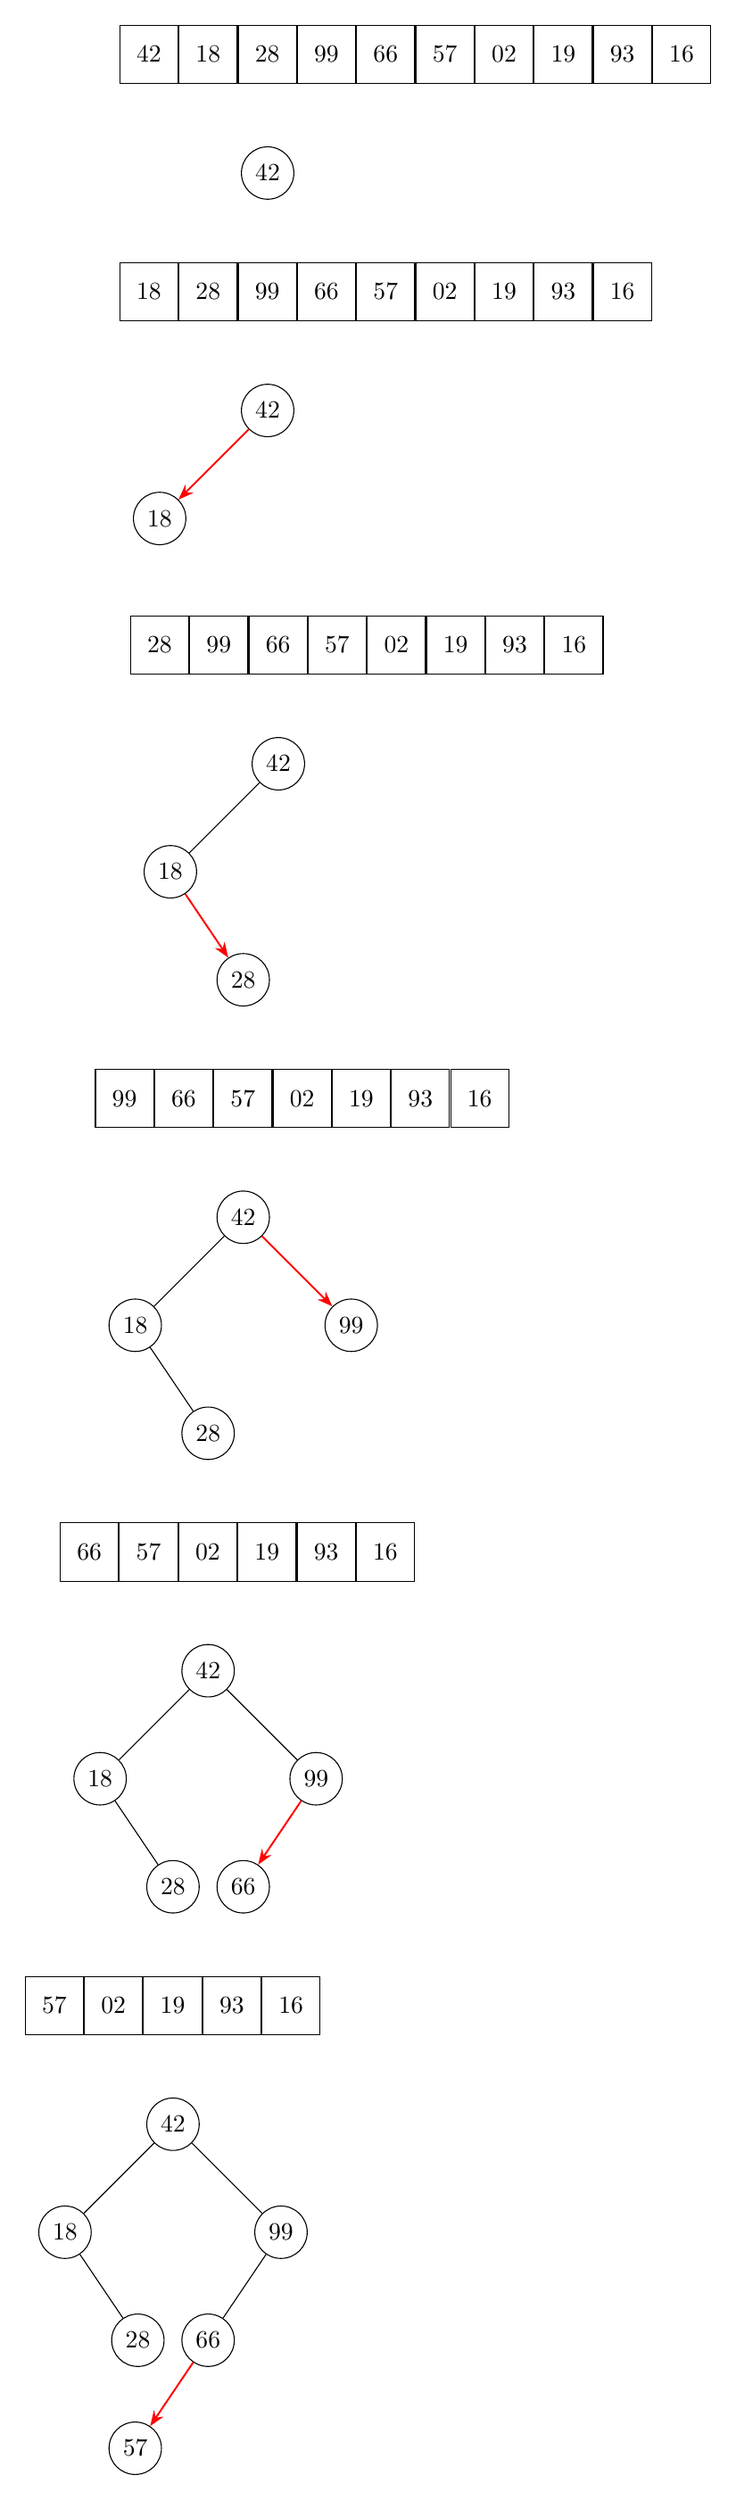
\begin{tikzpicture}
    \node[draw, square] (a) {42};
    \node[draw, square, right=0cm of a] (b) {18};
    \node[draw, square, right=0cm of b] (c) {28};
    \node[draw, square, right=0cm of c] (d) {99};
    \node[draw, square, right=0cm of d] (e) {66};
    \node[draw, square, right=0cm of e] (f) {57};
    \node[draw, square, right=0cm of f] (g) {02};
    \node[draw, square, right=0cm of g] (h) {19};
    \node[draw, square, right=0cm of h] (i) {93};
    \node[draw, square, right=0cm of i] (j) {16};

    \node[draw, circle, below right=of a] (root0) {42};


    \node[draw, square, below left= of root0] (b1) {18};
    \node[draw, square, right=0cm of b1] (c1) {28};
    \node[draw, square, right=0cm of c1] (d1) {99};
    \node[draw, square, right=0cm of d1] (e1) {66};
    \node[draw, square, right=0cm of e1] (f1) {57};
    \node[draw, square, right=0cm of f1] (g1) {02};
    \node[draw, square, right=0cm of g1] (h1) {19};
    \node[draw, square, right=0cm of h1] (i1) {93};
    \node[draw, square, right=0cm of i1] (j1) {16};

    \node[draw, circle, below right=of b1] (root1) {42};
    \node[draw, circle, below left=of root1] (node18_1) {18};

    \draw[myarrow, red] (root1) -- (node18_1);

    \node[draw, square, below= of node18_1](c2) {28};
    \node[draw, square, right=0cm of c2] (d2) {99};
    \node[draw, square, right=0cm of d2] (e2) {66};
    \node[draw, square, right=0cm of e2] (f2) {57};
    \node[draw, square, right=0cm of f2] (g2) {02};
    \node[draw, square, right=0cm of g2] (h2) {19};
    \node[draw, square, right=0cm of h2] (i2) {93};
    \node[draw, square, right=0cm of i2] (j2) {16};

    \node[draw, circle, below right=of c2] (root2) {42};
    \node[draw, circle, below left=of root2] (node18_2){18};
    \node[draw, circle, below right=of node18_2, xshift=-5mm] (node28_2) {28};

    \draw (root2) -- (node18_2);
    \draw[myarrow, red] (node18_2) -- (node28_2);

    \node[draw, square, below left= of node28_2] (d3) {99};
    \node[draw, square, right=0cm of d3] (e3) {66};
    \node[draw, square, right=0cm of e3] (f3) {57};
    \node[draw, square, right=0cm of f3] (g3) {02};
    \node[draw, square, right=0cm of g3] (h3) {19};
    \node[draw, square, right=0cm of h3] (i3) {93};
    \node[draw, square, right=0cm of i3] (j3) {16};

    \node[draw, circle, below right=of d3] (root3) {42};
    \node[draw, circle, below left=of root3] (node18_3){18};
    \node[draw, circle, below right=of root3] (node99_3){99};
    \node[draw, circle, below right=of node18_3, xshift=-5mm] (node28_3) {28};

    \draw (root3) -- (node18_3);
    \draw (node18_3) -- (node28_3);
    \draw[myarrow, red] (root3) -- (node99_3);

    \node[draw, square, below left= of node28_3] (e4) {66};
    \node[draw, square, right=0cm of e4] (f4) {57};
    \node[draw, square, right=0cm of f4] (g4) {02};
    \node[draw, square, right=0cm of g4] (h4) {19};
    \node[draw, square, right=0cm of h4] (i4) {93};
    \node[draw, square, right=0cm of i4] (j4) {16};

    \node[draw, circle, below right=of e4] (root4) {42};
    \node[draw, circle, below left=of root4] (node18_4){18};
    \node[draw, circle, below right=of root4] (node99_4){99};
    \node[draw, circle, below right=of node18_4, xshift=-5mm] (node28_4) {28};
    \node[draw, circle, below left=of node99_4, xshift=5mm] (node66_4) {66};

    \draw (root4) -- (node18_4);
    \draw (node18_4) -- (node28_4);
    \draw (root4) -- (node99_4);
    \draw[myarrow, red] (node99_4) -- (node66_4);

    \node[draw, square, below left= of node28_4] (f5) {57};
    \node[draw, square, right=0cm of f5] (g5) {02};
    \node[draw, square, right=0cm of g5] (h5) {19};
    \node[draw, square, right=0cm of h5] (i5) {93};
    \node[draw, square, right=0cm of i5] (j5) {16};

    \node[draw, circle, below right=of f5] (root5) {42};
    \node[draw, circle, below left=of root5] (node18_5){18};
    \node[draw, circle, below right=of root5] (node99_5){99};
    \node[draw, circle, below right=of node18_5, xshift=-5mm] (node28_5) {28};
    \node[draw, circle, below left=of node99_5, xshift=5mm] (node66_5) {66};
    \node[draw, circle, below left=of node66_5, xshift=5mm] (node57_5) {57};

    \draw (root5) -- (node18_5);
    \draw (node18_5) -- (node28_5);
    \draw (root5) -- (node99_5);
    \draw (node99_5) -- (node66_5);
    \draw[myarrow, red] (node66_5) -- (node57_5);
\end{tikzpicture}
\end{document}
